%
% slides.tex -- slides
%
% (c) 2017 Prof Dr Andreas Müller, Hochschule Rapperswil
%
\theoremstyle{definition}
\newtheorem{dgl}{Differentialgleichungen}
\newtheorem{dgl1}{Differentialgleichung}
\newtheorem{lsg}{Lösungen}
\newtheorem{anomalie}{Anomalie}
\newtheorem{zust}{Zustandsgleichung}
\newtheorem{zirk}{Zirkulationsrichtung}

\definecolor{darkgreen}{rgb}{0,0.5,0}

\begin{document}

\ifthenelse{\boolean{presentation}}{
\begin{frame}
\titlepage
\end{frame}

\begin{frame}
\frametitle{Förderband}
\begin{center}
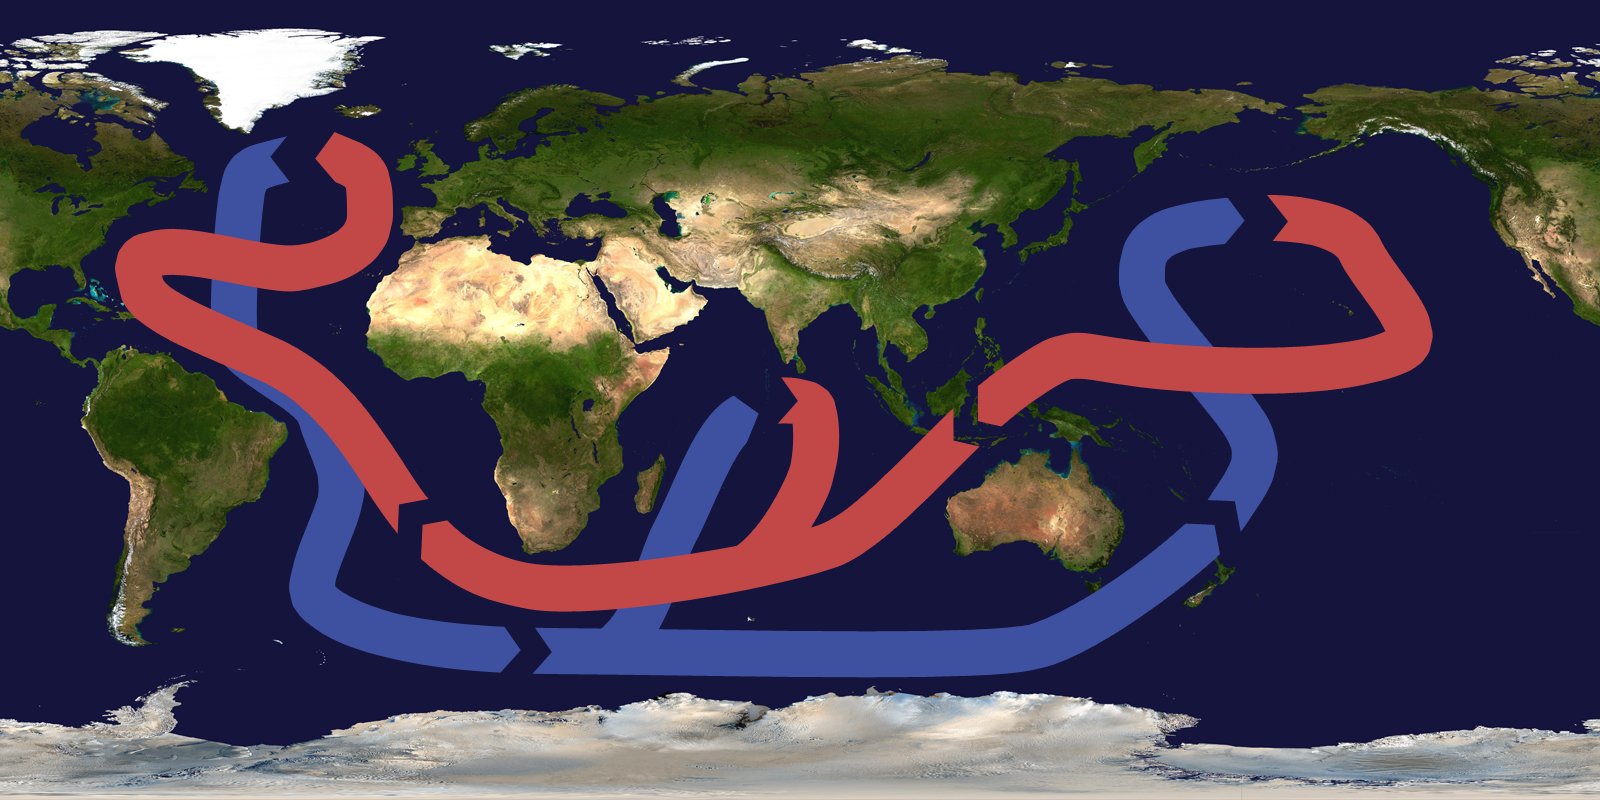
\includegraphics[width=\hsize]{../03_thc/Thermohaline_circulation.png}
\end{center}
\end{frame}

}

%
% Box-Modell
%
\begin{frame}
\frametitle{Box-Modell}
\begin{center}
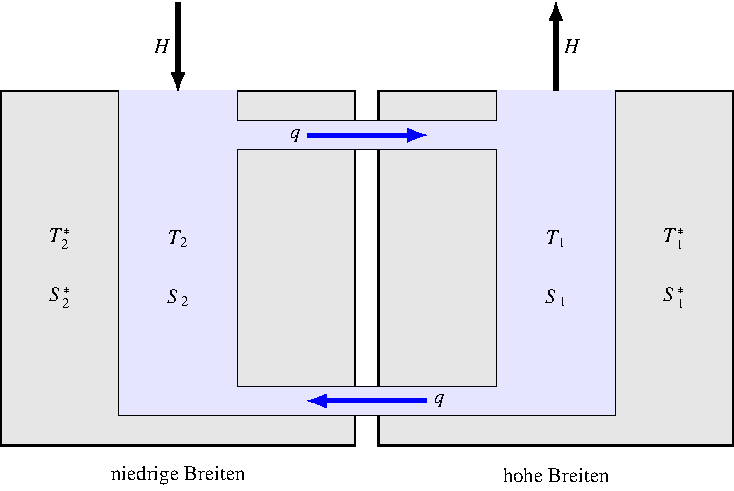
\includegraphics[width=0.8\textwidth]{../../skript/chapters/4/boxmodell.pdf}
\end{center}
\end{frame}

%
% Mittel-Temperatur und -Salinität
%
\begin{frame}
\frametitle{Mittel-Temperatur und -Salinität}
\begin{anomalie}
\vspace{-10pt}
\begin{align*}
T_0
&=
\frac{T_1+T_2}{2} - \frac{T_1^*+T_2^*}{2}
&
S_0
&=
\frac{S_1+S_2}{2} - \frac{S_1^*+S_2^*}{2}
\end{align*}
\end{anomalie}
\begin{dgl}
\vspace{-10pt}
\begin{align*}
\frac{d}{dt} T_0 &= -cT_0
&
\frac{d}{dt} S_0 &= -dS_0
\end{align*}
\end{dgl}
\begin{lsg}
\vspace{-10pt}
\begin{align*}
T_0(t) &= T_0(0) e^{-ct}
&
S_0(t) &= S_0(0) e^{-dt}
\end{align*}
$\Rightarrow$
Mitteltemperatur und -salinität gleichen sich exponentiell schnell an.
\end{lsg}
\end{frame}

%
% Temperatur- und Salinitäts-Differenz
%
\begin{frame}
\frametitle{Temperatur- und Salinitäts-Differenzen}
\begin{dgl}
Temperatur- und Salinitätsdifferenzen bestehen über lange Zeit:
\begin{align*}
\frac{d}{dt}\Delta T
&=
\phantom{2H+\mathstrut}
c(2T^* - \Delta T) -2|q|\Delta T
\\
\frac{d}{dt}\Delta S
&=
2H + d(2S^* - \Delta S) - 2|q|\Delta S
\end{align*}
\end{dgl}
\begin{zust}
Dichteunterschiede treiben die Zirkulation an:
\begin{align*}
\varrho
&=
\varrho_0
(1-\alpha (T-T_0) + \beta(S-S_0))
\\
q
&=
k\frac{\varrho_1-\varrho_2}{\varrho_0}
=
k(\alpha\Delta T - \beta \Delta S)
\end{align*}
\end{zust}
\end{frame}

%
% Vereinfachungen
%
\begin{frame}
\frametitle{Vereinfachungen}
\begin{enumerate}
\item
Thermische Prozesse sind schnell: $\Delta T = 2 T^*$
\item
Salinitätsangleichung ist langsam: $d=0$
\end{enumerate}
Verbleibende Gleichung:
\begin{align*}
\frac{d}{dt} \Delta S
&=
2H - 2|q|\Delta S
\\
&=
2H
-
2|\alpha T^* - \beta \Delta S| \Delta S
\intertext{Dimensionslos:}
\frac{d}{dt}
\frac{\beta\Delta S}{\alpha T^*}
&=
\frac{2\beta H}{\alpha T^*}
-2
\alpha T^{*}
\biggl|1-\frac{\beta\Delta S}{\alpha T^*}\biggr| \cdot \frac{\beta \Delta S}{\alpha T^*}
\\
\underbrace{
\frac{1}{\color{blue}2\alpha T^*}
\frac{d}{\color{blue}dt}
}_{\displaystyle\color{blue}\frac{d}{d\tau}}
\underbrace{
{\color{red} \frac{\beta\Delta S}{\alpha T^*}}}_{\displaystyle\color{red} x}
&=
\underbrace{
{\color{darkgreen} \frac{\beta H}{\alpha^2 T^{*2}}}
}_{\displaystyle\color{darkgreen} \lambda}
-
\biggl|1-
\underbrace{\color{red}\frac{\beta\Delta S}{\alpha T^*}}_{\displaystyle\color{red}x}\biggr|\cdot \underbrace{\color{red}\frac{\beta \Delta S}{\alpha T^*}}_{\displaystyle\color{red}x}
&
\color{blue}
\tau
&=
\color{blue}
2\alpha T^* t
\end{align*}
\end{frame}

%
% 
%
\begin{frame}
\frametitle{Bifurkation}
\vspace{-15pt}
\begin{columns}
\begin{column}{0.36\textwidth}
\begin{dgl1}
\vspace{-5pt}
\[
\dot x
=
\lambda - |1-x|x
\]
\end{dgl1}
hat Sattel-Knoten-Bifurkation bei $\lambda=\frac14$.

\begin{zirk}
Vorzeichen von $q$: $1-x$.

\begin{itemize}
\item
Sprung von $x<1$ zu $x>1$ bedeutet Umkehr der
thermohalinen Zirkulation
\item
Umkehr ist irreversibel
\end{itemize}
\end{zirk}

\end{column}
\begin{column}{0.6\textwidth}
\begin{center}
%
% drei.tex
%
% (c) 2018 Prof Dr Andreas Müller, Hochschule Rapperswil
%
\documentclass[tikz]{standalone}
\usepackage{times}
\usepackage{amsmath}
\usepackage{txfonts}
\usepackage[utf8]{inputenc}
\usepackage{graphics}
\usetikzlibrary{arrows,intersections}
\usetikzlibrary{math}
\begin{document}
\begin{tikzpicture}[thick, >= latex, xscale = 20, yscale = 6]

\draw[domain=0:0.5,samples=100,color=red]
	plot ({0.25 - (\x-0.5)*(\x-0.5)},{\x});

\draw[domain=0.5:1,samples=100,color=blue]
	plot ({0.25 - (\x-0.5)*(\x-0.5)},{\x});

\draw[domain=1:1.3,samples=100,color=red]
	plot ({(\x-0.5)*(\x-0.5)-0.25},{\x});

\draw[->] (-0.03,0)--(0.4,0) coordinate[label={above:$\lambda$}];
\draw[->] (0,-0.03)--(0,1.35) coordinate[label={right:$x$}];

\draw (-0.003,1)--(0.003,1);
\node at (-0.003,1) [left] {$1$};

\draw (0.25,-0.03)--(0.25,0.03);
\node at (0.25,-0.03) [below] {$\frac14$};

\node at (0.25,0.5) [right] {$S$};
\fill[color=red] (0.25,0.5) circle[x radius={0.07/20},y radius={0.07/6}];
\draw[color=red,line width=0.5] (0.25,0.5)--(0.25,{0.5+sqrt(0.5)});
\node at (0.25,{0.5+sqrt(0.5)}) [below right] {$P$};
\fill[color=red] (0.25,{0.5+sqrt(0.5)}) circle[x radius={0.07/20}, y radius={0.07/6}];

\end{tikzpicture}
\end{document}


\end{center}
\end{column}
\end{columns}
\end{frame}

\end{document}
